\chapter[Conclusão]{Conclusão}
\label{cap:conclusao}

% {aqui vai um parágrafo retomando objetivo e questão de pesquisa, porque fecha o TCC1}

\section{Atividades concluídas}
% {atividades do TCC1 realizadas, relacionadas aos objetivos específicos, porque mostra que o plano foi cumprido}

\section{Resultados obtidos}
% {principais achados da revisão e o planejamento concluído}

\section{Próximos passos}
% {o que será feito no TCC2, porque liga as duas etapas}

\section{Cronograma da segunda etapa}
% {tabela de atividades e meses do TCC2}
A segunda etapa da monografia consiste na execução integral do experimento planejado, no tratamento e análise dos dados obtidos e na redação da versão final do trabalho. O cronograma previsto é apresentado na Figura~\ref{fig:cronograma-etapa2}. 

Entre as principais atividades estão:


\begin{figure}[H]
  \centering
  \caption{Cronograma da segunda etapa}
  \label{fig:cronograma-etapa2}
  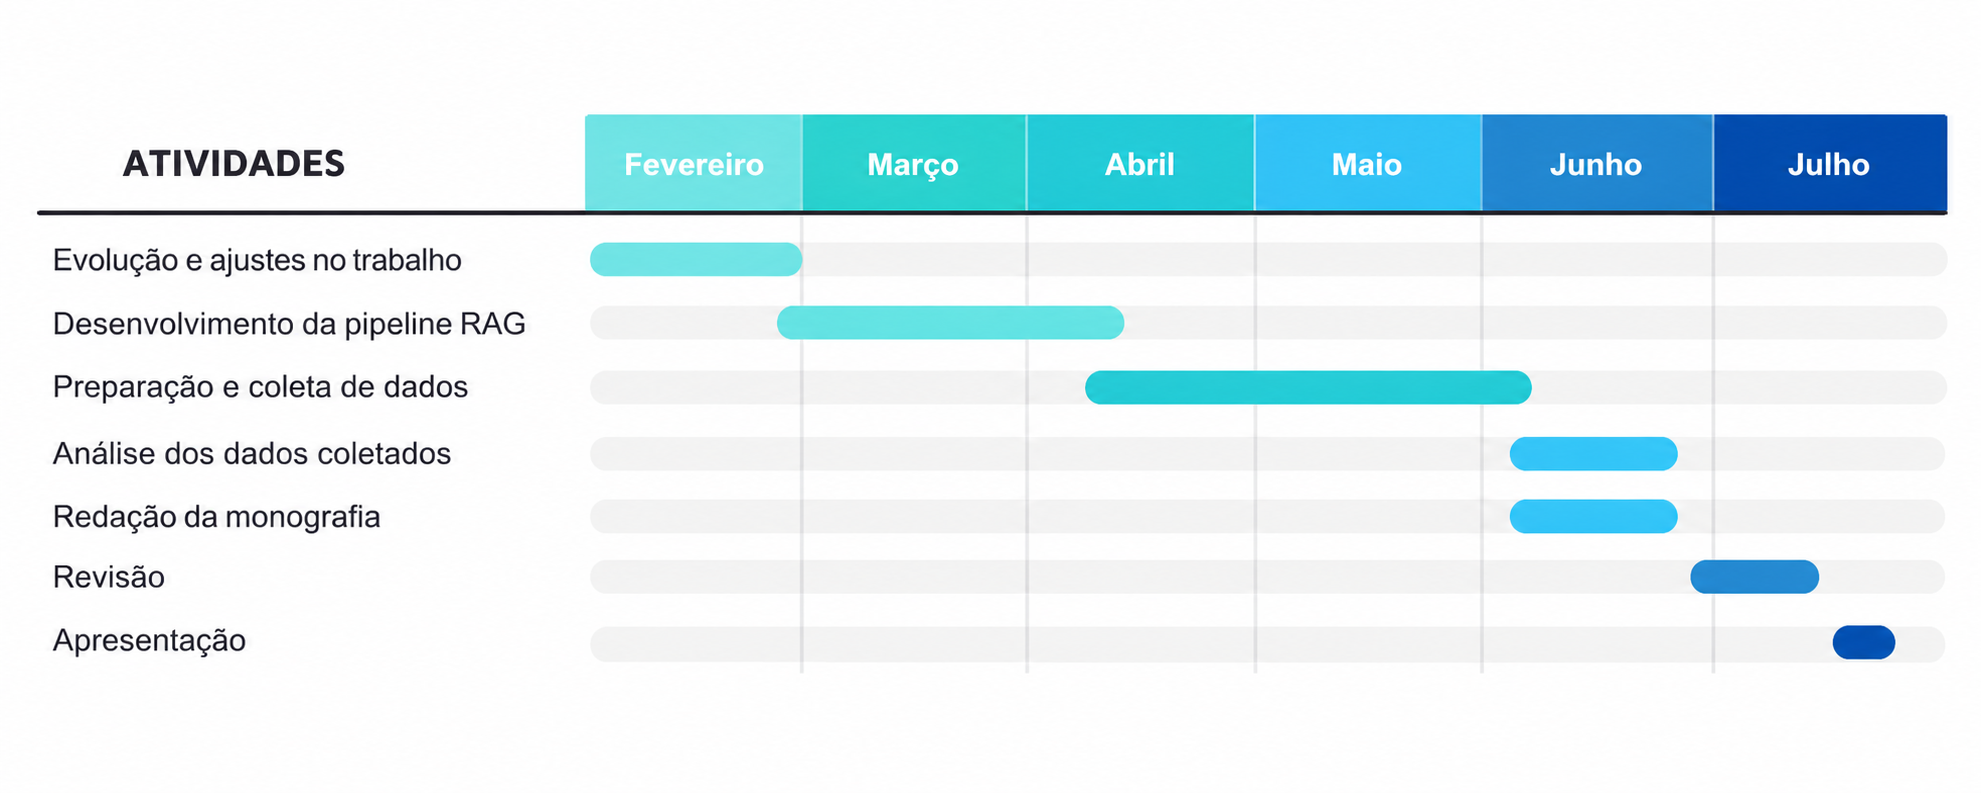
\includegraphics[width=\textwidth]{figuras/cronograma-etapa2.png}
  \fonte{Autores}
\end{figure}